% !TeX root = ./beamer.tex
%%%%%%%%%%%%%%%%%%%%%%%%%%%%%%%%%%%%%%%%%%%%%%%%%%%%%%%%%%%%%%%%%%%%%%
%
% Beamer template with UiT colour scheme
%
%%%%%%%%%%%%%%%%%%%%%%%%%%%%%%%%%%%%%%%%%%%%%%%%%%%%%%%%%%%%%%%%%%%%%%

\documentclass[xcolor=dvipsnames]{beamer} %
\usetheme[progressbar=frametitle,
	titleformat=smallcaps,
	% sectionpage=none,
	numbering=fraction,
	block=fill,
	background=dark]{metropolis}
\usefonttheme{professionalfonts}
\usefonttheme{serif} % default family is serif
\usetikzlibrary{arrows,shapes}
% If you want notes on the side:
% \setbeameroption{show notes on second screen=right} % Both
% \setbeamertemplate{note page}{\pagecolor{yellow!5}\vfill\insertnote\vfill}\usepackage{palatino}

\usepackage{utils/definitions}
\usepackage{utils/divide_toc}
\usepackage{utils/beamerouterthemesplit}
\usepackage{utils/citecmd}
\usepackage{utils/footfix}
\usepackage{utils/colors}
\setbeamerfont{footnote}{size=\tiny}

\title[Chemistry in CESM2]{Chemistry in CESM2}
\author{\textsc{Eirik Rolland Enger}}
\date{\vspace{-3mm}December 9, 2022\hfill
\includegraphics[width=4cm]{utils/CSU-Official-wrdmrk-Rev-2.png}}
\logo{\vspace{-2mm}
\includegraphics[width=15mm]{utils/CSU-Official-wrdmrk-Rev-2.png}\hspace{1mm}}
% \institute{UiT --- The Arctic University of Norway}
\begin{document}
\maketitle

% For every picture that defines or uses external nodes, you'll have to
% apply the 'remember picture' style. To avoid some typing, we'll apply
% the style to all pictures.
\tikzstyle{every picture}+=[remember picture]
% By default all math in TikZ nodes are set in inline mode. Change this to
% displaystyle so that we don't get small fractions.
\everymath{\displaystyle}

\begin{frame}%,[allowframebreaks]
	\frametitle{Overview}

	\setbeamertemplate{section in toc}[sections numbered]
	\tableofcontents[hideallsubsections]

\end{frame}

\section{Motivation}

\subsection{SSW}
\begin{frame}{Stratospheric Sudden Warmings}
	\begin{itemize}
		\item Defined as a wind reversal at $ \SI{10}{\hecto\pascal} $ $ (\sim\SI{25}{\kilo\metre}) $
	\end{itemize}
\end{frame}

\begin{frame}{Stratospheric Sudden Warmings}
	\begin{center}
		\copyrightbox[r]{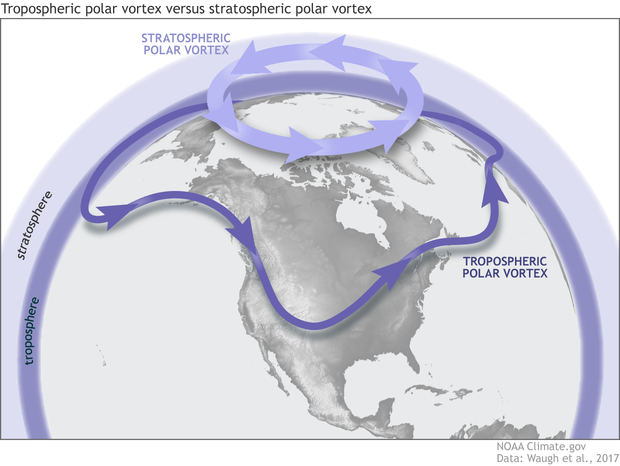
\includegraphics[width=0.85\linewidth]{./assets/Polar-Vortex.png}}
		{\tiny\href{https://www.climate.gov/news-features/blogs/enso/polar-vortex-going-make-you-put-sweater-be-afraid-be-very-afraid#:~:text=Thus\%2C\%20the\%20tropospheric\%20polar\%20vortex,that\%20separates\%20the\%20air\%20masses.}{Image from climate.gov}}
	\end{center}
\end{frame}

\subsection{QBO}
\begin{frame}{Quasi-Bilennial Oscillation}
	Internally generated QBO
\end{frame}

\subsection{Ozone}
\begin{frame}{Evolution of the Ozone layer}
	\begin{itemize}
		\item WACCM6 is able to reproduce the evolution of the ozone layer (also SH polar ozone hole)
		\item Lower stratospheric ozone field is dynamically controlled, and vertical
		      velocity will impact the total column ozone
	\end{itemize}
\end{frame}

\subsection{Sea Ice}
\begin{frame}{Sea Ice}
	The September NH sea ice extent is better in WACCM6 than in CAM6

	Less downward surface SW and LW in WACCM6 due to higher LWP\footnote{liquid
		water path} which in turn is due to higher aerosol number

	$ \Rightarrow $ Tropospheric aerosol chemistry impacts Arctic sea ice

	\begin{center}
		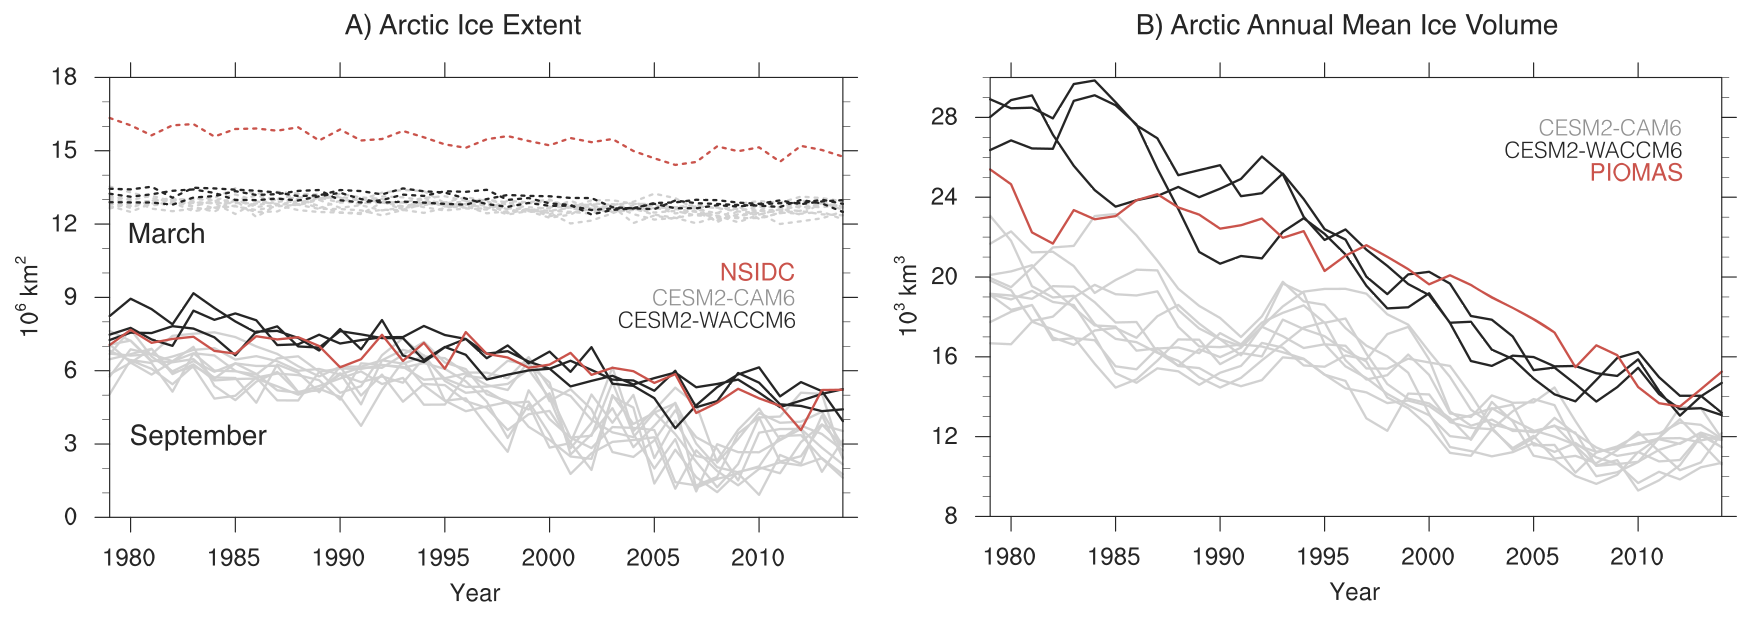
\includegraphics[width=0.95\linewidth]{./assets/ice-extent3.png}
	\end{center}

\end{frame}

\subsection{Atmospheric Blocking}
\begin{frame}{Atmospheric Blocking}
	\scriptsize
	Frequency of the meridional gradient of 500-hPa geopotential height below a
	threshold of $ \mathrm{GHGS}>0$, $\mathrm{GHGN}<\SI{-5}{\metre/degree} $
	\begin{align*}
		\mathrm{GHGS} & =\frac{Z(\phi_0)-Z(\phi_{\mathrm{S}})}{\phi_0-\phi_{\mathrm{S}}} \\
		\mathrm{GHGN} & =\frac{Z(\phi_{\mathrm{N}})-Z(\phi_0)}{\phi_\mathrm{N}-\phi_0}
		\label{eq:blocking-frequency}
	\end{align*}
	where \(\phi_{\mathrm{N}}=\SI{78.75}{\degree N}+\Delta\),
	\(\phi_{0}=\SI{60}{\degree N}+\Delta\), \(\phi_{\mathrm{S}}=\SI{41.25}{\degree N}+\Delta\)
	and \(\Delta=\SI{-3.75}{\degree},\SI{0}{\degree},\SI{3.75}{\degree}\).\cite{dandrea1998}

    Stratospherical dynamical processees important for high-latitude tropospheric
    climate variability.
\end{frame}

\section{Differences}

\begin{frame}{First: Similarities}
	\begin{itemize}
		\item Top of atmosphere energy budget
		\item Cloud radiative effects
		\item Tropospheric physical processes are the same in CAM6 and WACCM6
	\end{itemize}
\end{frame}

\begin{frame}{Closer to observation}
	\begin{itemize}
		\item September Northern Hemisphere sea ice extent
	\end{itemize}
\end{frame}

\subsection{Spatial}
\begin{frame}{Spatial}
	\begin{itemize}
		\item Top goes from $ \SI{40}{\kilo\metre} $ to $ \SI{140}{\kilo\metre} $
		\item Vertical resolution is somewhat similar in the troposphere
		\item Horizontal resolution is the same?
	\end{itemize}
\end{frame}

\subsection{Chemistry}
\begin{frame}{Chemistry}
	Empty
\end{frame}

\begin{frame}{Stratospheric Aerosols}
	For example, in CAM, stratospheric aerosols are prescribed based on output from
	previous WACCM simulations
    \begin{figure}
        \begin{center}
            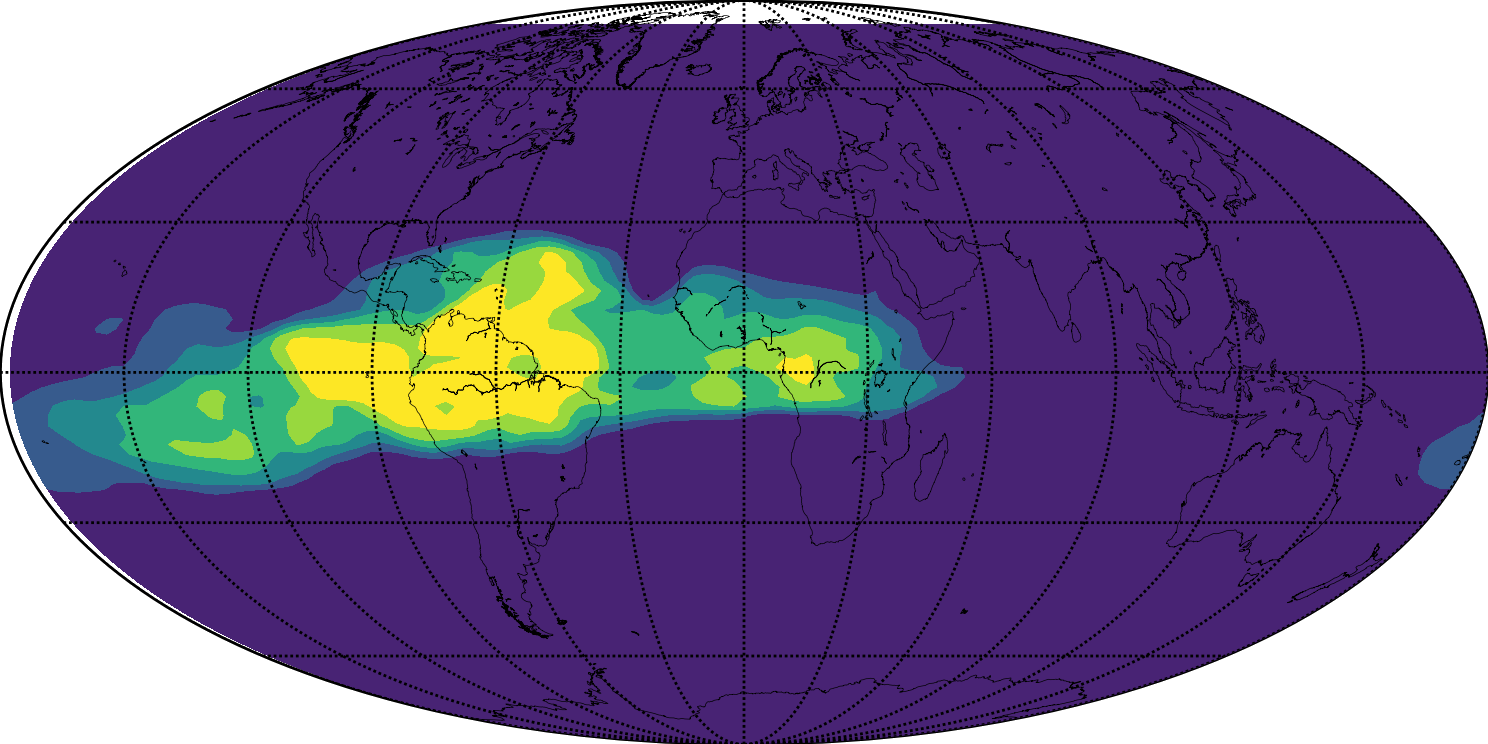
\includegraphics[width=0.95\textwidth]{./assets/frame_00009-2.png}
        \end{center}
        \label{fig:so2-distribution}
    \end{figure}
\end{frame}

\begin{frame}{CAM Default Chemistry}
	A blanket of aerosols if you want to simulate them.
\end{frame}

\section{Additions}

\begin{frame}{D-region}
	Space physics, even one that goes up to $ \SI{500}{\kilo\metre} $ (WACCM6-X)
\end{frame}

\subsection{How high}
\begin{frame}
	\frametitle{First frame}
\end{frame}

\subsection{When}
\begin{frame}
	\frametitle{Second frame}
\end{frame}

\subsection{sub2}
\begin{frame}
	\frametitle{Second frame}
\end{frame}

\section{Chemical Reactions}

\subsection{Basic}
\begin{frame}{Basics}
	Nothing.
\end{frame}

\begin{frame}{Lumping}
	Molecules are lumped together based on how similar they are, for example to reduce computation costs.
	(See for example Emmons et al. 2020, sec. 2.3.)
\end{frame}

\begin{frame}{Reactions in MOZART}
	See \href{https://agupubs.onlinelibrary.wiley.com/action/downloadSupplement?doi=10.1029\%2F2019MS001882&file=jame21103-sup-0003-2019MS001882+Table_SI-S02.pdf}{table 2}\footnote{
		\url{https://agupubs.onlinelibrary.wiley.com/action/downloadSupplement?doi=10.1029\%2F2019MS001882&file=jame21103-sup-0003-2019MS001882+Table_SI-S02.pdf}}
	for a complete list of chemical reactions included in CESM2 when run with the TSMLT
	(troposphere, stratosphere, mesossphere, lower thermosphere) configuration.
\end{frame}

\section{Use cases}

\subsection{Aerosol spread}
\begin{frame}{\texorpdfstring{\ce{SO2}}{SO2} to Aerosols}
	Here is an animation!
\end{frame}

\begin{frame}{Final Remarks}
	Finally.
\end{frame}

\begin{frame}{Future Projects}
	List of stuff.
\end{frame}

\appendix

% \section{Appendix}
% \input{underscript/appendix.tex}
\nocite{gettleman2019}
\nocite{mills2016}
\nocite{mills2017}
\nocite{marsh2007}
\nocite{marsh2013}
\nocite{garcia2007}
\begin{frame}[allowframebreaks,plain]{References}

	\printbibliography[heading=none]

\end{frame}

\end{document}
